% ============================================================
%  Chapter 2 -- Theoretical Background
% ============================================================
\chapter{Theoretical Background}
\label{ch:background}

This chapter develops the theoretical foundations required to understand
the contributions of this thesis.
We begin with the mathematical machinery of deep learning
(Section~\ref{sec:deep-learning-foundations}),
then trace the evolution of learned representations from 1D audio to
2D images to 3D point clouds
(Section~\ref{sec:signal-progression}).
We cover 3D geometric representations and their properties
(Section~\ref{sec:3d-representations}),
compression theory and the principal point cloud codecs
(Section~\ref{sec:compression}),
the specific deep learning tools used in this work
(Section~\ref{sec:deep-learning-3d}),
and the quality metrics employed throughout
(Section~\ref{sec:metrics}).

\section{Foundations of Deep Learning}
\label{sec:deep-learning-foundations}

\subsection{Artificial Neural Networks}

An artificial neural network (ANN) is a parameterised function
$f_\theta : \mathcal{X} \to \mathcal{Y}$ composed of layers of simple
computational units called neurons.
A single neuron with $d$-dimensional input $\mathbf{x} \in \R^d$ computes:
\begin{equation}
  z = \sigma\!\left(\mathbf{w}^\top \mathbf{x} + b\right), \quad
  \mathbf{w} \in \R^d,\ b \in \R,
\end{equation}
where $\mathbf{w}$ is a weight vector, $b$ a bias scalar, and $\sigma$ a
non-linear \emph{activation function}.
The activation function is what prevents the network from collapsing to a
single linear transformation regardless of depth; popular choices are the
Rectified Linear Unit (ReLU, $\sigma(z) = \max(0, z)$), sigmoid
($\sigma(z) = 1/(1+e^{-z})$), and hyperbolic tangent
($\sigma(z) = \tanh(z) \in (-1, 1)$).

Arranging neurons into $L$ sequential \emph{layers} gives a multi-layer
perceptron (MLP):
\begin{equation}
  \mathbf{h}^{(0)} = \mathbf{x}, \qquad
  \mathbf{h}^{(\ell)} = \sigma\!\left(\mathbf{W}^{(\ell)} \mathbf{h}^{(\ell-1)}
    + \mathbf{b}^{(\ell)}\right), \qquad \ell = 1, \ldots, L,
\end{equation}
where $\mathbf{W}^{(\ell)} \in \R^{d_\ell \times d_{\ell-1}}$ and
$\mathbf{b}^{(\ell)} \in \R^{d_\ell}$.
The final layer produces the network output $f_\theta(\mathbf{x}) = \mathbf{h}^{(L)}$.
The universal approximation theorem~\cite{cybenko1989approximation,hornik1989multilayer} guarantees
that a sufficiently wide single-hidden-layer MLP can approximate any continuous
function on a compact domain, but depth --- not just width --- is the key
practical enabler of modern networks.
Figure~\ref{fig:mlp} illustrates a three-layer MLP with the information flow
from input to output.

\begin{figure}[t]
\centering
\begin{tikzpicture}[
  >=Stealth,
  neuron/.style={circle, draw, minimum size=0.50cm, inner sep=0pt, line width=0.6pt},
]
  \def\layersep{2.0cm}
  \def\vsep{0.62cm}
  % Input (4): y = (1.5-i)*vsep for i=0..3  => 0.93, 0.31, -0.31, -0.93
  \foreach \i in {0,...,3}
    \node[neuron, fill=blue!18, draw=blue!50]       (I\i) at (0,           {(1.5-\i)*\vsep}) {};
  % Hidden (5): y = (2-i)*vsep for i=0..4  => 1.24, 0.62, 0, -0.62, -1.24
  \foreach \i in {0,...,4}
    \node[neuron, fill=green!18, draw=green!55]     (H\i) at (\layersep,   {(2-\i)*\vsep})   {};
  % Output (3): y = (1-i)*vsep for i=0..2  => 0.62, 0, -0.62
  \foreach \i in {0,...,2}
    \node[neuron, fill=red!15,  draw=red!45]        (O\i) at (2*\layersep, {(1-\i)*\vsep})   {};
  % Connections
  \foreach \i in {0,...,3}
    \foreach \j in {0,...,4}
      \draw[gray!45, very thin] (I\i) -- (H\j);
  \foreach \i in {0,...,4}
    \foreach \j in {0,...,2}
      \draw[gray!45, very thin] (H\i) -- (O\j);
  % Layer labels — placed well above the top neuron of each column
  % Input top at y = 0.93+0.25 = 1.18; label at 1.50
  \node[font=\small\bfseries, blue!65]        at (0,           1.52) {Input};
  % Hidden top at y = 1.24+0.25 = 1.49; label at 1.85
  \node[font=\small\bfseries, green!60!black] at (\layersep,   1.87) {Hidden};
  % Output top at y = 0.62+0.25 = 0.87; label aligned with Input
  \node[font=\small\bfseries, red!65]         at (2*\layersep, 1.52) {Output};
  % Activation formula below hidden column
  % Hidden bottom at y = -1.24-0.25 = -1.49
  \node[font=\footnotesize] at (\layersep, -1.78)
    {$\mathbf{h}^{(\ell)} = \sigma\!\left(\mathbf{W}^{(\ell)}\mathbf{h}^{(\ell-1)}+\mathbf{b}^{(\ell)}\right)$};
\end{tikzpicture}
\caption{%
  A multi-layer perceptron (MLP) with one hidden layer.
  Every neuron in each layer connects to every neuron in the next
  (fully-connected); a non-linear activation $\sigma$ is applied
  element-wise after each linear transformation.
}
\label{fig:mlp}
\end{figure}

\subsection{Training via Backpropagation and Gradient Descent}

Training a neural network amounts to finding parameters $\theta^*$ that minimise
an empirical loss $\mathcal{L}(\theta)$ over a dataset
$\{(\mathbf{x}_i, \mathbf{y}_i)\}_{i=1}^N$:
\begin{equation}
  \theta^* = \arg\min_\theta \frac{1}{N}\sum_{i=1}^N
    \ell\!\left(f_\theta(\mathbf{x}_i),\, \mathbf{y}_i\right),
\end{equation}
where $\ell$ is a per-sample loss (e.g., mean squared error for regression,
cross-entropy for classification).

Gradient descent updates parameters in the direction of steepest loss decrease:
\begin{equation}
  \theta \leftarrow \theta - \eta \,\nabla_\theta \mathcal{L}(\theta),
\end{equation}
where $\eta > 0$ is the learning rate.
In practice, stochastic gradient descent (SGD) approximates the full gradient
using a random mini-batch $\mathcal{B} \subset \{1,\ldots,N\}$ at each step,
dramatically reducing per-step computation while retaining convergence
guarantees under mild conditions.

The critical insight that makes training deep networks feasible is
\emph{backpropagation}~\cite{lecun1989backpropagation}: an efficient
application of the chain rule that computes the gradient of the loss with
respect to all parameters in a single backward pass, at computational cost
proportional to the forward pass.
For a scalar loss $\mathcal{L}$ and a composed function $f = f_L \circ \cdots \circ f_1$,
the gradient with respect to the parameters of layer $\ell$ is:
\begin{equation}
  \frac{\partial \mathcal{L}}{\partial \mathbf{W}^{(\ell)}} =
    \frac{\partial \mathcal{L}}{\partial \mathbf{h}^{(L)}}
    \cdot \frac{\partial \mathbf{h}^{(L)}}{\partial \mathbf{h}^{(L-1)}}
    \cdots \frac{\partial \mathbf{h}^{(\ell+1)}}{\partial \mathbf{h}^{(\ell)}}
    \cdot \frac{\partial \mathbf{h}^{(\ell)}}{\partial \mathbf{W}^{(\ell)}}.
\end{equation}
Modern deep learning frameworks (PyTorch, TensorFlow) implement automatic
differentiation to compute these gradients without user intervention.

\subsection{Adaptive Optimisers}

Plain SGD applies a uniform learning rate to all parameters.
Adam~\cite{kingma2015adam} improves on this by maintaining
per-parameter first and second moment estimates of the gradients:
\begin{align}
  \mathbf{m}_t &= \beta_1 \mathbf{m}_{t-1} + (1-\beta_1)\mathbf{g}_t, \\
  \mathbf{v}_t &= \beta_2 \mathbf{v}_{t-1} + (1-\beta_2)\mathbf{g}_t^2, \\
  \hat{\mathbf{m}}_t &= \mathbf{m}_t / (1 - \beta_1^t), \quad
  \hat{\mathbf{v}}_t = \mathbf{v}_t / (1 - \beta_2^t), \\
  \theta_t &= \theta_{t-1} - \eta\, \hat{\mathbf{m}}_t / (\sqrt{\hat{\mathbf{v}}_t} + \epsilon).
\end{align}
AdamW~\cite{loshchilov2017decoupled} decouples weight decay from the gradient
update by adding a direct $\ell_2$ penalty on weights:
\begin{equation}
  \theta_t = (1 - \eta\lambda)\theta_{t-1}
    - \eta\, \hat{\mathbf{m}}_t / (\sqrt{\hat{\mathbf{v}}_t} + \epsilon),
\end{equation}
where $\lambda$ is the weight decay coefficient.
Decoupling weight decay from the adaptive gradient scaling corrects a
regularisation inconsistency in the original Adam update and generally
improves generalisation.

\subsection{Regularisation, Overfitting, and Learning Rate Schedules}

A model with enough capacity will memorise the training set
(\emph{overfitting}): training loss decreases but the function fails to
generalise.
The most direct remedy is to constrain the effective function class.
\emph{Weight decay} ($\ell_2$ regularisation) adds $\lambda\|\theta\|_2^2$
to the loss, penalising large weights and biasing the optimiser toward smoother
solutions.
\emph{Dropout}~\cite{srivastava2014dropout} randomly zeroes a fraction $p$
of activations during training, preventing units from co-adapting and
effectively training an ensemble of sub-networks.

For spatial tasks, \emph{data augmentation} is often the most
cost-effective regulariser.
Label-preserving transforms --- rotations, flips, scale jitter --- expand
the effective training distribution without new labels.
In this work all 48 discrete symmetries of the 3D
cube~\cite{winkels2018gcnn,cohen2016equivariant} are applied uniformly to
point cloud patches, exploiting the fact that codec distortions are
invariant to the orientation and reflection of the patch.
\emph{Batch normalisation}~\cite{ioffe2015batch} standardises intermediate
activations within each mini-batch; beyond reducing internal covariate shift,
it stabilises training and has a regularising effect that reduces sensitivity
to the learning rate.
Training is terminated by \emph{early stopping} when held-out validation
loss stops improving.

A fixed learning rate is rarely optimal.
A high rate accelerates early training but prevents convergence to a sharp
minimum; a low rate is too slow from a random initialisation.
In this work the two are combined: the rate is increased linearly from
$10^{-5}$ to the peak $10^{-3}$ over the first few epochs (\emph{linear
warm-up}), preventing large gradient steps from destabilising batch statistics
before they have stabilised, then follows a cosine
schedule~\cite{loshchilov2017sgdr}:
\begin{equation}
  \eta_t = \eta_{\min} + \tfrac{1}{2}(\eta_{\max} - \eta_{\min})
           \bigl(1 + \cos(\pi t / T)\bigr),
\end{equation}
gradually decreasing to $\eta_{\min}$ over $T$ epochs.
The smooth decay allows fine-grained convergence in the later epochs without
premature stalling.


% ============================================================

\section{From 1D Signals to 3D Geometry: Evolution of Representation Learning}
\label{sec:signal-progression}

\subsection{1D Signals: Audio Processing and Sequential Data}

Audio waveforms were the first domain where the interplay between
sampling theory, transform design, and perceptual coding was worked out
rigorously, and the same ideas recur in 2D and 3D.
The Nyquist-Shannon sampling theorem~\cite{shannon1949noise} establishes
the foundational link between continuous and discrete representations:
a bandlimited signal $x(t)$ with maximum frequency $f_{\max}$ is perfectly
reconstructable from its samples $x[n]$ provided the sampling rate exceeds
$2f_{\max}$.
Without this result, the entire chain from ADC to digital storage to playback
is undefined.

Traditional audio codecs (MP3, AAC) exploit the mismatch between signal
information content and the resolution of human auditory perception.
The Modified Discrete Cosine Transform (MDCT)~\cite{princen1987mdct} decomposes overlapping frames
into frequency subbands; coefficients in less perceptually sensitive bands
are quantised more coarsely; the result is entropy-coded.
Designing the perceptual weighting functions required decades of
psychoacoustic research.

Deep learning replaced hand-crafted transforms with learned ones.
WaveNet~\cite{oord2016wavenet} modelled the raw audio waveform
autoregressively using dilated causal convolutions with exponentially growing
receptive fields, generating high-quality speech.
HiFi-GAN~\cite{kong2020hifigan} applied a generative adversarial network (GAN)
trained directly on waveforms to achieve real-time high-fidelity synthesis.
The core operation in all these systems is the 1D convolution:
a kernel $\mathbf{w} \in \R^k$ slides over the sequence
$x[n]$ to produce:
\begin{equation}
  y[n] = \sum_{i=0}^{k-1} w[i] \cdot x[n - i].
\end{equation}
Dilation by factor $d$ skips samples:
$y[n] = \sum_{i=0}^{k-1} w[i] \cdot x[n - d\cdot i]$,
exponentially expanding the receptive field without proportionally increasing
the parameter count.

\subsection{2D Signals: Image Understanding and Convolutional Networks}

Images extend 1D signals to a 2D regular grid $x[m, n]$ of pixel intensities.
The Discrete Cosine Transform (DCT), applied blockwise, underpins JPEG
compression; the H.264/H.265 family adds inter-frame motion compensation for
video.
Both systems are built on expert-crafted transforms: the DCT was chosen
for its energy-compaction properties; motion estimation is heuristic.

The revolution in image understanding came from \emph{learning} the transforms
directly from data.
A 2D convolution slides a learnable kernel
$\mathbf{W} \in \R^{k \times k \times C_{in} \times C_{out}}$
over the input to produce feature maps:
\begin{equation}
  y_{c'}[m, n] = \sum_{c=1}^{C_{in}} \sum_{i=-\lfloor k/2\rfloor}^{\lfloor k/2\rfloor}
    \sum_{j=-\lfloor k/2\rfloor}^{\lfloor k/2\rfloor}
    W_{c,c'}[i, j] \cdot x_c[m+i,\, n+j].
\end{equation}
The key structural property is \emph{weight sharing}: the same kernel is
applied at every spatial location, reducing parameter count from $O(N^2)$
to $O(k^2 C_{in} C_{out})$ relative to a fully connected layer.
A direct consequence is \emph{translation equivariance}: shifting the input
shifts the output by the same amount, so the network does not need to
re-learn a detector at every position.
Figure~\ref{fig:conv2d} illustrates the $3\times 3$ convolution operation.

\begin{figure}[t]
\centering
\begin{tikzpicture}[>=Stealth]
  \def\cs{0.56}  % cell size
  % ---- 5x5 input grid ----
  \foreach \i in {0,...,4}
    \foreach \j in {0,...,4} {
      \pgfmathsetmacro\clr{int(18+mod(\i*7+\j*11,20))}
      \fill[blue!\clr!white] ({\j*\cs},{-\i*\cs}) rectangle ++({\cs},{\cs});
      \draw[gray!50, very thin] ({\j*\cs},{-\i*\cs}) rectangle ++({\cs},{\cs});
    }
  % Receptive field: rows i=1..3, cols j=1..3 — fully inside the grid
  % x: [cs, 4*cs] = [0.56, 2.24];  grid x: [0, 5*cs=2.80]  ✓
  % y: [-3*cs, 0] = [-1.68, 0];    grid y: [-4*cs=-2.24, cs=0.56]  ✓
  \draw[red!80, very thick, rounded corners=1pt]
    ({\cs},{-3*\cs}) rectangle ++({3*\cs},{3*\cs});
  \node[font=\small, below] at ({2.5*\cs},{-5*\cs-0.06}) {Input $\mathbf{x}$};

  % Convolution symbol — at the vertical centre of the 5x5 grid
  \node[font=\large] at ({5*\cs+0.45},{-1.5*\cs}) {$*$};

  % ---- 3x3 kernel (yshift=-\cs centres it on the 5x5 input) ----
  \begin{scope}[xshift={5*\cs cm + 0.85cm}, yshift={-\cs cm}]
    \foreach \i in {0,...,2}
      \foreach \j in {0,...,2} {
        \fill[orange!28] ({\j*\cs},{-\i*\cs}) rectangle ++({\cs},{\cs});
        \draw[orange!60] ({\j*\cs},{-\i*\cs}) rectangle ++({\cs},{\cs});
        \node[font=\tiny] at ({\j*\cs+0.5*\cs},{-\i*\cs+0.5*\cs}) {$w_{\i\j}$};
      }
    \node[font=\small, below] at ({1.5*\cs},{-4*\cs-0.06}) {Kernel $\mathbf{w}$};
  \end{scope}

  % Equals sign
  \node[font=\large] at ({5*\cs+0.85+3*\cs+0.45},{-1.5*\cs}) {$=$};

  % ---- 3x3 output grid (yshift=-\cs centres it on the 5x5 input) ----
  \begin{scope}[xshift={5*\cs cm + 0.85cm + 3*\cs cm + 0.85cm}, yshift={-\cs cm}]
    \foreach \i in {0,...,2}
      \foreach \j in {0,...,2} {
        \fill[green!18] ({\j*\cs},{-\i*\cs}) rectangle ++({\cs},{\cs});
        \draw[green!55!black] ({\j*\cs},{-\i*\cs}) rectangle ++({\cs},{\cs});
      }
    % Highlighted output cell corresponding to the RF (row 1, col 1)
    \fill[green!55] ({\cs},{-\cs}) rectangle ++({\cs},{\cs});
    \node[font=\small, below] at ({1.5*\cs},{-4*\cs-0.06}) {Output $\mathbf{y}$};
  \end{scope}
\end{tikzpicture}
\caption{%
  A $3{\times}3$ convolution on a $5{\times}5$ input feature map.
  The kernel (orange) slides over the input, computing a dot product at each
  position to produce one output value (green).
  The highlighted receptive field (red border) shows the input region that
  contributes to one output position.
}
\label{fig:conv2d}
\end{figure}

Stacking convolutional layers with interleaved non-linearities and spatial
downsampling (max pooling, strided convolution) builds a hierarchy of features
whose receptive field grows with depth.
AlexNet~\cite{krizhevsky2012alexnet} was the first to demonstrate on ImageNet that this learned
hierarchy dramatically outperforms hand-crafted feature pipelines; VGG,
GoogLeNet, and ResNet~\cite{he2016deep} subsequently showed that depth and
efficient skip-connection design were the main levers for further gains.

The key architectural innovation that made very deep networks trainable was
the residual block.
Instead of learning a mapping $\mathbf{H}(\mathbf{x})$ from input to output,
a residual block learns the residual $\mathbf{F}(\mathbf{x}) = \mathbf{H}(\mathbf{x}) - \mathbf{x}$
and adds the identity:
\begin{equation}
  \mathbf{H}(\mathbf{x}) = \mathbf{F}(\mathbf{x}) + \mathbf{x}.
\end{equation}
This reformulation makes it easy for the network to learn the identity mapping
(by setting $\mathbf{F} = \mathbf{0}$), which ensures that adding more layers
cannot hurt performance.
Residual connections also provide a direct gradient path from the output to
early layers, alleviating the vanishing gradient problem.

For dense prediction tasks (segmentation, depth estimation, image restoration),
the output resolution must match the input.
U-Net~\cite{ronneberger2015unet} introduced the encoder-decoder with skip
connections: an encoder path progressively downsamples with strided
convolutions (or pooling), building a compact high-level representation;
a symmetric decoder path progressively upsamples; at each resolution level,
skip connections concatenate encoder features to decoder inputs, preserving
fine-scale spatial detail.
\begin{equation}
  \mathbf{h}^{(dec)}_\ell = f_\ell^{dec}\!\left(
    [\,\mathbf{h}^{(enc)}_\ell\, ;\, \text{upsample}(\mathbf{h}^{(dec)}_{\ell+1})\,]\right),
\end{equation}
where $[\cdot\,;\,\cdot]$ denotes channel concatenation.

Learned compression extended the same encoder-decoder idea to the
rate-distortion problem.
Ballé et al.~\cite{balle2018variational} replaced the hand-crafted DCT
with a learned CNN encoder-decoder and introduced the \emph{hyperprior}:
a second entropy model that codes the scale parameters of the main latent
distribution, capturing spatial correlations in the quantised latent.
Minnen et al.~\cite{minnen2018joint} added an autoregressive prior that
conditions each latent element on previously decoded context, further
improving entropy coding efficiency.
These systems now surpass JPEG-2000 on standard benchmarks and provided
the blueprint for learned point cloud codecs (Section~\ref{sec:compression}).

\subsection{3D Data: Geometric Representations and the Sparsity Challenge}

Extending image-like deep learning to 3D confronts an immediate structural
problem: the spatial data is \emph{sparse and irregular}.
A $512 \times 512$ image contains exactly $262\,144$ pixels in a regular grid.
The same scene at the same spatial resolution in 3D would occupy a
$512^3 \approx 134\,\text{M}$ voxel grid, of which fewer than 1\% are
occupied by surface points.
Applying standard 3D convolutions at this resolution requires $\sim$512 GB
of memory for feature maps at a modest 64 channels --- clearly impractical.

Processing only the occupied subset requires representations that make
sparsity explicit rather than storing an empty grid.
The three principal approaches to this are surveyed in
Section~\ref{sec:3d-representations}.


% ============================================================

\section{Point Cloud Geometry}
\label{sec:3d-representations}

\subsection{Definition and Properties}

A point cloud $\pc = \{p_i\}_{i=1}^{N}$ is an unordered finite set of
points $p_i = (x_i, y_i, z_i) \in \R^3$, each optionally augmented with
attribute vectors $a_i \in \R^d$ (colour, surface normal, reflectance).
This work focuses exclusively on geometry (coordinates); attributes are not
used.

Three properties of point clouds distinguish them from images and meshes.
First, the set is \emph{unordered}: any permutation of the points produces
the same geometric object, so a deep learning model must produce outputs that
are permutation invariant (for global tasks such as classification) or
permutation equivariant (for per-point tasks such as segmentation or
displacement prediction).
Second, points are \emph{irregular}: they are not at fixed grid positions,
so standard convolutions, which assume a regular grid, cannot be applied
directly.
Third, point clouds are \emph{variable in size}: different frames or objects
may contain vastly different numbers of points, requiring architectures that
handle variable input lengths.

\paragraph{Early approaches: PointNet.}
The first architecture to handle permutation invariance explicitly was
PointNet~\cite{qi2017pointnet}.
It processes each point independently through a shared MLP, then aggregates
all per-point features via a symmetric function (global max pooling):
\begin{equation}
  f(\{p_1, \ldots, p_N\}) = g\!\left(\max_{i=1}^N h(p_i)\right),
\end{equation}
where $h$ is the shared per-point MLP and $g$ is a further transformation.
Global max pooling is both permutation invariant and differentiable.
PointNet++ \cite{qi2017pointnetplusplus} extended this with a hierarchical
local grouping mechanism, enabling the network to capture local geometric
context at multiple scales.

\subsection{Comparison with Meshes and Voxel Grids}

Three main 3D representations compete in practice:

\paragraph{Voxel grids.}
The bounding box is divided into a regular $G^3$ lattice, and each cell
is labelled occupied or empty.
Voxel grids support standard 3D convolutions directly and are easy to
process; their fundamental weakness is cubic scaling with resolution.
At resolution $G = 1024$ (used by the 8iVFB dataset), a naive binary
occupancy grid requires $1024^3 / 8 \approx 128$\,MB per frame even before
feature storage.

\paragraph{Polygonal meshes.}
A mesh represents a surface as a set of vertices $V \subset \R^3$ connected
by a set of faces $F$ (typically triangles).
Meshes are compact for smooth surfaces and support efficient rendering.
Their weaknesses are: difficult to acquire directly from sensors (requiring
a reconstruction step); sensitive to mesh connectivity irregularities;
and hard to process with standard neural architectures.
Graph convolutional networks~\cite{wang2019dynamic} address the connectivity
challenge but scale poorly to the hundreds of thousands of faces in
high-quality captures.

\paragraph{Point clouds.}
Point clouds are acquired directly by LiDAR and structured-light sensors,
require no reconstruction step, and represent geometry without connectivity
assumptions.
They scale linearly with the number of occupied surface points $N$,
not cubically with resolution.
Their principal weakness is the lack of a canonical neighbourhood structure,
which makes local processing non-trivial.

For the large-scale volumetric captures in this work, point clouds
\emph{voxelized} to integer grid positions provide the best balance:
they retain the sparsity advantage of point sets while enabling efficient
sparse convolutional processing.

\subsection{Voxelization and Sparse Tensors}
\label{ssec:voxelization}

Voxelization maps point cloud coordinates to integer grid positions at a
fixed resolution $G$:
\begin{equation}
  p_i = (x_i, y_i, z_i) \longmapsto
    \left\lfloor \frac{p_i - p_{\min}}{p_{\max} - p_{\min}} \cdot G \right\rceil
    \in \{0, \ldots, G-1\}^3.
\end{equation}
Multiple points mapping to the same voxel are merged (typically by taking
the mean attribute value or simply marking the voxel occupied).

The resulting structure is a \emph{sparse tensor}: a tensor that stores
values only at a small subset of its index space.
Formally, a sparse tensor $\mathbf{F}$ is defined by:
\begin{itemize}
  \item A coordinate matrix $\mathbf{C} \in \mathbb{Z}^{N \times 3}$ of $N$
    active (occupied) voxel positions.
  \item A feature matrix $\mathbf{F} \in \R^{N \times C}$ assigning a
    $C$-dimensional vector to each active voxel.
\end{itemize}
MinkowskiEngine~\cite{choy20194d} implements generalised sparse
convolutions on this data structure, enabling U-Net architectures to run
directly on point clouds at $O(N)$ cost (Section~\ref{ssec:sparse-conv}).
Figure~\ref{fig:voxelization} illustrates the voxelization process and the
sparsity structure of the resulting tensor.

\begin{figure}[t]
\centering
\resizebox{0.90\linewidth}{!}{%
\begin{tikzpicture}[>=Stealth]
  \def\gs{0.42}  % voxel cell size

  % ---- Left: continuous point cloud ----
  \foreach \x/\y in {0.25/2.05, 0.50/2.20, 0.78/2.30, 1.05/2.22,
                      1.30/2.00, 1.55/1.68, 1.78/1.30, 1.98/0.90,
                      2.12/0.55, 2.22/0.28} {
    \fill[blue!55] (\x, \y) circle (2.0pt);
  }
  \node[font=\small, below] at (1.2, 0.02) {Point cloud};
  \draw[->, thick, gray!60] (2.55, 1.15) -- node[above, font=\footnotesize]{voxelise} (3.35, 1.15);

  % ---- Middle: 6x6 voxel grid ----
  \begin{scope}[xshift=3.6cm]
    \foreach \i in {0,...,5}
      \foreach \j in {0,...,5}
        \draw[gray!28, very thin] ({\i*\gs},{\j*\gs}) rectangle ++({\gs},{\gs});
    % Occupied voxels corresponding to the arc
    \foreach \i/\j in {0/4, 1/4, 1/5, 2/5, 3/4, 3/5, 4/3, 5/2} {
      \fill[blue!32] ({\i*\gs},{\j*\gs}) rectangle ++({\gs},{\gs});
      \draw[blue!50, thin] ({\i*\gs},{\j*\gs}) rectangle ++({\gs},{\gs});
    }
    \node[font=\small, below] at ({3*\gs}, 0.02) {Voxelised};
    \node[font=\tiny, red!60, below] at ({3*\gs}, -0.28) {8/36 occupied};
    \draw[->, thick, gray!60]
      ({6*\gs+0.18}, {3*\gs})
      -- node[above, font=\footnotesize]{encode}
      ({6*\gs+0.90}, {3*\gs});
  \end{scope}

  % ---- Right: sparse tensor (C and F as side-by-side table, no overlap) ----
  \begin{scope}[xshift=7.50cm]
    \node[draw, rounded corners=4pt, fill=gray!6,
          minimum width=3.0cm, inner sep=6pt] at (1.3, 1.30) {%
      \begin{tabular}{@{}c|c@{}}
        \multicolumn{2}{@{}c@{}}{\small\textbf{Sparse tensor}}\\[2pt]
        \scriptsize$\mathbf{C}\;(N{\times}3)$ & \scriptsize$\mathbf{F}\;(N{\times}C)$\\
        \hline
        \scriptsize\texttt{(0,4)} & \scriptsize$\mathbf{f}^{(1)}$\\
        \scriptsize\texttt{(1,4)} & \scriptsize$\mathbf{f}^{(2)}$\\
        \scriptsize$\vdots$       & \scriptsize$\vdots$
      \end{tabular}%
    };
  \end{scope}
\end{tikzpicture}%
}
\caption{%
  Voxelization converts a continuous point cloud (left) to an integer-coordinate
  sparse tensor (centre, right).
  Each occupied voxel becomes one row in the coordinate matrix $\mathbf{C}$ paired
  with a feature row in $\mathbf{F}$.
  Unoccupied voxels are not stored, giving $O(N)$ memory for a surface with
  $N \ll G^3$ points.
}
\label{fig:voxelization}
\end{figure}

\subsection{Surface Curvature Estimation}
\label{ssec:curvature-theory}

Surface curvature at a point $p$ quantifies the local deviation of the surface
from a plane.
In the discrete point cloud setting, curvature is estimated from the local
neighbourhood $\mathcal{N}_k(p)$ of the $k$ nearest neighbours.

\paragraph{Covariance analysis.}
The local covariance matrix is:
\begin{equation}
  \mathbf{C}(p) = \frac{1}{k}\sum_{q \in \mathcal{N}_k(p)}
    (q - \bar{p})(q - \bar{p})^\top \in \R^{3\times3},
  \qquad \bar{p} = \frac{1}{k}\sum_{q \in \mathcal{N}_k(p)} q.
\end{equation}
The eigenvectors of $\mathbf{C}(p)$ approximate the local surface frame:
the eigenvector corresponding to the smallest eigenvalue $\lambda_0$ aligns
with the surface normal; the other two span the tangent plane.

\paragraph{Surface variation.}
The surface variation descriptor~\cite{pauly2002efficient}:
\begin{equation}
  \kappa(p) = \frac{\lambda_0}{\lambda_0 + \lambda_1 + \lambda_2} \in [0, 1]
\end{equation}
approximates normalised curvature.
For a perfectly flat region, $\lambda_0 = 0$ and $\kappa = 0$.
For an isotropic corner with equal variation in all directions,
$\lambda_0 = \lambda_1 = \lambda_2$ and $\kappa = 1/3$.
In practice, values above $0.05$ typically correspond to visually detectable
edges or ridges.

The choice of $k$ controls the spatial scale of the curvature estimate.
Too small a $k$ yields noisy estimates dominated by scan-point jitter;
too large a $k$ smooths over fine geometric features.
We use $k = 30$ throughout, which captures neighbourhood geometry at the
scale of fine surface features in 8iVFB clouds voxelized at $G = 1024$.

Figure~\ref{fig:curvature-stratification} illustrates the curvature estimation
and stratification procedure.

\begin{figure}[t]
\centering
\resizebox{0.96\linewidth}{!}{%
\begin{tikzpicture}[>=Stealth,
  pstep/.style={draw, rounded corners=4pt, inner sep=8pt, align=center,
                font=\small, minimum width=2.6cm, minimum height=0.72cm},
  arr/.style={->, thick, gray!55},
]
  % Pipeline steps
  \node[pstep, fill=blue!8,  draw=blue!30]   (s1) at (0.0, 0)
    {$k$-NN\\{\scriptsize $k{=}30$ neighbours}};
  \node[pstep, fill=blue!13, draw=blue!35]   (s2) at (3.6, 0)
    {Covariance\\{\scriptsize $\mathbf{C}(p_i) \in \mathbb{R}^{3\times 3}$}};
  \node[pstep, fill=blue!18, draw=blue!40]   (s3) at (7.2, 0)
    {Eigenvalues\\{\scriptsize $\lambda_0 \leq \lambda_1 \leq \lambda_2$}};
  \node[pstep, fill=blue!23, draw=blue!50]   (s4) at (10.8, 0)
    {Surface variation\\{\scriptsize $\kappa = \lambda_0 / \sum_j \lambda_j$}};

  % Input label
  \node[font=\small, left] at (s1.west) {$\mathcal{P}$\enspace};

  % Stratum outputs
  \node[pstep, fill=green!12, draw=green!45, minimum width=3.4cm] (flat) at (8.2, -2.8)
    {Flat stratum\\{\scriptsize $\kappa \leq \kappa_{33}$}};
  \node[pstep, fill=red!12,   draw=red!45,   minimum width=3.4cm] (edge) at (12.4, -2.8)
    {Edge stratum\\{\scriptsize $\kappa > \kappa_{67}$}};

  % Flow arrows
  \draw[arr] (s1) -- node[above, font=\tiny]{k-NN} (s2);
  \draw[arr] (s2) -- node[above, font=\tiny]{PCA}   (s3);
  \draw[arr] (s3) -- node[above, font=\tiny]{ratio}  (s4);
  \draw[arr] (s4.south) -- ++(0,-1.2) -| (flat.north);
  \draw[arr] (s4.south) -- ++(0,-1.2) -| (edge.north);
\end{tikzpicture}%
}
\caption{%
  Curvature estimation and stratification pipeline.
  For each point, the $k$-nearest neighbours are found, a local covariance
  matrix is computed, and the surface variation $\kappa$ is estimated from
  the smallest eigenvalue ratio.
  Points are then partitioned into flat (lower tercile) and edge (upper tercile)
  strata using percentile thresholds computed on the original point cloud.
}
\label{fig:curvature-stratification}
\end{figure}

\subsection{Applications and Datasets}

Point cloud processing is central to several application domains of societal
and commercial relevance:

\begin{description}
  \item[Autonomous driving.]
    Vehicle-mounted LiDAR sensors (Velodyne HDL-64E, Ouster OS1~\cite{roriz2022lidar}) produce
    continuous dense outdoor scans at 10--20 fps.
    These clouds are used for 3D object detection, semantic segmentation,
    simultaneous localisation and mapping (SLAM), and path planning.
    The sparsity profile is very different from volumetric video:
    road scenes are large, sparsely sampled, with many thin structures
    (poles, pedestrians).

  \item[Volumetric video / immersive telepresence.]
    Multi-camera capture rigs reconstruct human bodies as dense, coloured
    point clouds for immersive video communication and extended reality.
    The \textit{8i Voxelized Full Bodies (8iVFB)} dataset~\cite{8ivfb} used in
    this work consists of four sequences (\textit{longdress}, \textit{loot},
    \textit{redandblack}, \textit{soldier}) acquired at 10 fps, containing
    300 frames per sequence at resolution $G = 1024$ with up to 800\,000
    points per frame.

  \item[Cultural heritage and digital preservation.]
    Structured-light scanners and photogrammetric pipelines preserve artefacts
    at sub-millimetre precision.
    Notable examples include scans of the Notre-Dame de Paris cathedral
    (used for reconstruction after the 2019 fire) and museum artefact
    digitisation programmes.

  \item[Medical imaging.]
    CT and MRI volumetric reconstructions can be converted to surface point
    clouds for surgical planning, prosthesis fitting, and anatomical
    analysis.

  \item[Robotics and industrial inspection.]
    Structured-light depth cameras (Intel RealSense, Microsoft Azure Kinect)
    produce dense point clouds for grasping, navigation, and quality control
    in manufacturing.
\end{description}

\subsection{The Microsoft Voxelized Upper Bodies (MVUB) Dataset}

The MVUB dataset~\cite{loop2016mvub} provides point clouds of human
upper bodies at resolution $G = 512$, acquired at 30 fps.
The subjects \textit{david10} and \textit{ricardo10} provide 10 frames each.
MVUB's lower resolution and different acquisition setup make it a useful
out-of-distribution test for generalisation experiments
(Section~\ref{ssec:mvub}).


% ============================================================

\section{Point Cloud Compression}
\label{sec:compression}

\subsection{Rate-Distortion Theory}
\label{ssec:rate-distortion}

Lossy compression is governed by the rate-distortion
function~\cite{shannon1959coding} $R(D)$: the minimum number of bits per
symbol required to represent a source with expected distortion at most $D$.
For a Gaussian source with quadratic distortion,
$R(D) = \frac{1}{2}\log_2(\sigma^2/D)$ bits per sample.
More generally, $R(D)$ is a non-increasing convex function of $D$:
lower distortion always requires higher rate.

\paragraph{Operational rate-distortion.}
A practical compression system cannot achieve the Shannon bound exactly;
it operates at some point $(R, D)$ on or above the theoretical curve.
Modern learned codecs optimise a Lagrangian:
\begin{equation}
  \mathcal{L} = \mathbb{E}\left[d(\mathbf{x}, \hat{\mathbf{x}})\right]
              + \lambda \cdot \mathbb{E}\left[-\log_2 p(\hat{\mathbf{y}})\right],
  \label{eq:rd-lagrangian}
\end{equation}
where the first term is the reconstruction distortion, the second is the
expected rate (cross-entropy under the entropy model), and $\lambda > 0$
controls the rate-distortion tradeoff.
Training a family of models at different $\lambda$ values traces out a
rate-distortion curve.
Lower $\lambda$ prioritises quality (high rate); higher $\lambda$ prioritises
compactness (high distortion).

\paragraph{Entropy coding.}
Given a probability model $p(\hat{\mathbf{y}})$, arithmetic coding achieves
a code length arbitrarily close to the Shannon entropy $-\sum_y p(y)\log_2 p(y)$.
In learned codecs, the entropy model is itself a neural network, trained
jointly with the encoder and decoder to minimise the bound in
Equation~\ref{eq:rd-lagrangian}.

\begin{figure}[t]
\centering
\begin{tikzpicture}[>=Stealth]
  % Plot region: 5.8cm wide, 3.8cm tall
  \def\W{5.8}
  \def\H{3.8}

  % Subtle background and border
  \fill[gray!4] (0,0) rectangle (\W,\H);
  \draw[gray!30] (0,0) rectangle (\W,\H);

  % Light horizontal grid lines
  \foreach \y in {0.95, 1.90, 2.85}
    \draw[gray!18] (0,\y) -- (\W,\y);

  % R-D curve: high quality at low rate, sweeping to high compression
  % Points carefully chosen to be on the curve interior, not clipped
  \draw[blue!65, very thick, smooth]
    plot[tension=0.45] coordinates {
      (0.30,3.50) (0.80,2.90) (1.50,2.25) (2.40,1.70)
      (3.40,1.28) (4.30,0.98) (5.30,0.72)
    }
    node[right, font=\small, blue!70] {$R(D)$};

  % Operating points
  \fill[red!60] (0.80, 2.90) circle (3.5pt);
  \fill[red!60] (2.40, 1.70) circle (3.5pt);
  \fill[red!60] (4.30, 0.98) circle (3.5pt);

  \node[font=\scriptsize, above right=-1pt] at (0.80, 2.90) {$\lambda_1$};
  \node[font=\scriptsize, above right=-1pt] at (2.40, 1.70) {$\lambda_2$};
  \node[font=\scriptsize, above right=-1pt] at (4.30, 0.98) {$\lambda_3$};

  % Annotation: direction of increasing lambda
  \draw[->, gray!50] (0.80, -0.52) -- (4.30, -0.52);
  \node[font=\tiny, gray!60] at (2.55, -0.72) {increasing $\lambda$ (more compression)};

  % Axes
  \draw[->] (0,0) -- (\W+0.40, 0) node[right, font=\small] {Rate (bpp)};
  \draw[->] (0,0) -- (0, \H+0.30) node[above, font=\small] {Quality (PSNR)};
\end{tikzpicture}
\caption{%
  Rate-distortion curve schematic.
  Training a codec at different Lagrange multipliers $\lambda$ traces
  different operating points on the rate-distortion curve: lower $\lambda$
  emphasises distortion reduction (high quality, high rate); higher $\lambda$
  emphasises bit savings (low quality, low rate).
  The curve represents the theoretical achievable boundary; practical
  systems operate on or above it.
}
\label{fig:rd-curve-concept}
\end{figure}

\subsection{Traditional Geometry Codecs}

\paragraph{G-PCC (Geometry-based Point Cloud Compression)~\cite{graziosi2020gpcc}.}
G-PCC is the MPEG geometry codec standard (ISO/IEC 23090-9).
It encodes geometry via recursive octree decomposition: the bounding box
is halved in each dimension until each leaf node contains at most one point.
At each octree level, the occupancy of the eight child nodes is represented
as an 8-bit symbol and arithmetic-coded using a probability model that
conditions on the parent and sibling context.

An alternative \emph{Trisoup} mode approximates the surface within each
leaf node by a planar triangle, enabling efficient coding of smooth surfaces
at low rates where fine voxel detail would be costly.

G-PCC does not introduce spatial bias: its artifacts manifest as
approximately uniform quantisation noise across the surface, independent
of local surface geometry.
This is the key qualitative difference from learned codecs, exploited in
the comparison in Chapter~\ref{ch:oversmoothing}.

\begin{figure}[t]
\centering
% Oblique-projection 3D octree (1.25× scale): x→right, y→upper-right, z→up
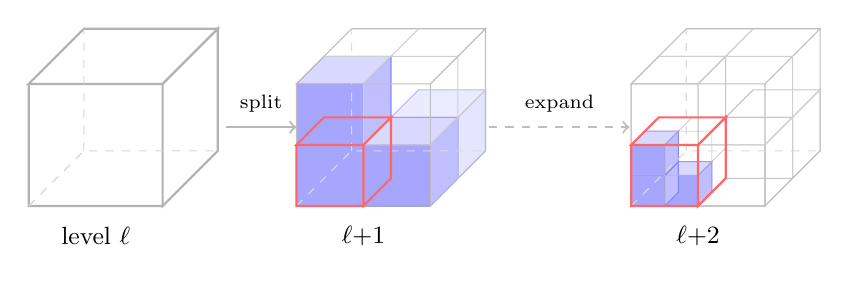
\begin{tikzpicture}[
  x={(0.85cm,0cm)}, y={(0.35cm,0.35cm)}, z={(0cm,0.775cm)},
  font=\small
]

% ── Panel 1: level-ℓ bounding box (outline only) ───────────────
\draw[gray!60, thick]
  (0,0,0)--(2,0,0)--(2,0,2)--(0,0,2)--cycle
  (2,0,0)--(2,2,0)--(2,2,2)--(2,0,2)--cycle
  (0,0,2)--(2,0,2)--(2,2,2)--(0,2,2)--cycle;
\draw[gray!32, dashed]
  (0,0,0)--(0,2,0)--(2,2,0)  (0,2,0)--(0,2,2);
\node[font=\small] at (0.85cm,-0.38cm) {level $\ell$};

% ── Arrow 1 ─────────────────────────────────────────────────────
\draw[->, thick, gray!55] (2.50cm,1.00cm)--(3.40cm,1.00cm);
\node[font=\scriptsize, above] at (2.95cm,1.06cm) {split};

% ── Panel 2: level-(ℓ+1), 4 occupied octants (painter order) ───
% Cube at (5,1,0) [back, draw first]
\fill[blue!15,draw=blue!38,thin]
  (5,1,0)--(6,1,0)--(6,1,1)--(5,1,1)--cycle;   % front
\fill[blue!10,draw=blue!32,thin]
  (6,1,0)--(6,2,0)--(6,2,1)--(6,1,1)--cycle;   % right
\fill[blue!8, draw=blue!28,thin]
  (5,1,1)--(6,1,1)--(6,2,1)--(5,2,1)--cycle;   % top
% Cube at (4,0,0)
\fill[blue!35,draw=blue!55,thin]
  (4,0,0)--(5,0,0)--(5,0,1)--(4,0,1)--cycle;   % front
\fill[blue!25,draw=blue!48,thin]
  (5,0,0)--(5,1,0)--(5,1,1)--(5,0,1)--cycle;   % right
\fill[blue!15,draw=blue!40,thin]
  (4,0,1)--(5,0,1)--(5,1,1)--(4,1,1)--cycle;   % top
% Cube at (5,0,0)
\fill[blue!35,draw=blue!55,thin]
  (5,0,0)--(6,0,0)--(6,0,1)--(5,0,1)--cycle;   % front
\fill[blue!25,draw=blue!48,thin]
  (6,0,0)--(6,1,0)--(6,1,1)--(6,0,1)--cycle;   % right
\fill[blue!15,draw=blue!40,thin]
  (5,0,1)--(6,0,1)--(6,1,1)--(5,1,1)--cycle;   % top
% Cube at (4,0,1) [top-front, last]
\fill[blue!35,draw=blue!55,thin]
  (4,0,1)--(5,0,1)--(5,0,2)--(4,0,2)--cycle;   % front
\fill[blue!25,draw=blue!48,thin]
  (5,0,1)--(5,1,1)--(5,1,2)--(5,0,2)--cycle;   % right
\fill[blue!15,draw=blue!40,thin]
  (4,0,2)--(5,0,2)--(5,1,2)--(4,1,2)--cycle;   % top
% Outer box
\draw[gray!50,thin]
  (4,0,0)--(6,0,0)--(6,0,2)--(4,0,2)--cycle
  (6,0,0)--(6,2,0)--(6,2,2)--(6,0,2)--cycle
  (4,0,2)--(6,0,2)--(6,2,2)--(4,2,2)--cycle;
\draw[gray!28,dashed]
  (4,0,0)--(4,2,0)--(6,2,0)  (4,2,0)--(4,2,2);
\draw[gray!38,thin]
  (5,0,0)--(5,0,2)   (5,0,2)--(5,2,2)
  (4,0,1)--(6,0,1)   (6,0,1)--(6,2,1)
  (6,1,0)--(6,1,2)   (4,1,2)--(6,1,2);
% Highlight the octant being expanded (front-bottom-left)
\draw[red!60, thick]
  (4,0,0)--(5,0,0)--(5,0,1)--(4,0,1)--cycle
  (5,0,0)--(5,1,0)--(5,1,1)--(5,0,1)--cycle
  (4,0,1)--(5,0,1)--(5,1,1)--(4,1,1)--cycle;
\node[font=\small] at (4.25cm,-0.38cm) {$\ell{+}1$};

% ── Arrow 2: Panel 2 right = 5.80cm; Panel 3 left = 7.65cm ─────
\draw[->, thick, gray!50, dashed] (5.84cm,1.00cm)--(7.63cm,1.00cm);
\node[font=\scriptsize, above] at (6.74cm,1.06cm) {expand};

% ── Panel 3: level-(ℓ+2), same 2×2×2 size as Panel 2 ──────────
% Red octant (9,0,0)-(10,1,1) shown subdivided in context.
% Surrounding 3 octants: outline only (ℓ+1 context, not ℓ+2 content).
% Sub-octants (0.5-unit) inside red octant: LR-Bot, LL-Bot, LL-Top.
% Painter order: back outline → bottom sub-octants → right outline
%                → top sub-octant → top outline → box/grid → red border

% Back octant (10,1,0): outline only
\draw[gray!45,thin]
  (10,1,0)--(11,1,0)--(11,1,1)--(10,1,1)--cycle
  (11,1,0)--(11,2,0)--(11,2,1)--(11,1,1)--cycle
  (10,1,1)--(11,1,1)--(11,2,1)--(10,2,1)--cycle;

% LR-Bot sub-octant (9.5,0,0)-(10,0.5,0.5): draw before front-right cube
\fill[blue!35,draw=blue!55,thin]
  (9.5,0,0)--(10,0,0)--(10,0,0.5)--(9.5,0,0.5)--cycle;   % front
\fill[blue!25,draw=blue!48,thin]
  (10,0,0)--(10,0.5,0)--(10,0.5,0.5)--(10,0,0.5)--cycle;   % right
\fill[blue!15,draw=blue!40,thin]
  (9.5,0,0.5)--(10,0,0.5)--(10,0.5,0.5)--(9.5,0.5,0.5)--cycle;   % top

% LL-Bot sub-octant (9,0,0)-(9.5,0.5,0.5)
\fill[blue!35,draw=blue!55,thin]
  (9,0,0)--(9.5,0,0)--(9.5,0,0.5)--(9,0,0.5)--cycle;     % front
\fill[blue!25,draw=blue!48,thin]
  (9.5,0,0)--(9.5,0.5,0)--(9.5,0.5,0.5)--(9.5,0,0.5)--cycle;   % right
\fill[blue!15,draw=blue!40,thin]
  (9,0,0.5)--(9.5,0,0.5)--(9.5,0.5,0.5)--(9,0.5,0.5)--cycle;   % top

% Front-right octant (10,0,0): outline only
\draw[gray!45,thin]
  (10,0,0)--(11,0,0)--(11,0,1)--(10,0,1)--cycle
  (11,0,0)--(11,1,0)--(11,1,1)--(11,0,1)--cycle
  (10,0,1)--(11,0,1)--(11,1,1)--(10,1,1)--cycle;

% LL-Top sub-octant (9,0,0.5)-(9.5,0.5,1): draw before front-top cube
\fill[blue!35,draw=blue!55,thin]
  (9,0,0.5)--(9.5,0,0.5)--(9.5,0,1)--(9,0,1)--cycle;     % front
\fill[blue!25,draw=blue!48,thin]
  (9.5,0,0.5)--(9.5,0.5,0.5)--(9.5,0.5,1)--(9.5,0,1)--cycle;   % right
\fill[blue!15,draw=blue!40,thin]
  (9,0,1)--(9.5,0,1)--(9.5,0.5,1)--(9,0.5,1)--cycle;     % top

% Front-top octant (9,0,1): outline only
\draw[gray!45,thin]
  (9,0,1)--(10,0,1)--(10,0,2)--(9,0,2)--cycle
  (10,0,1)--(10,1,1)--(10,1,2)--(10,0,2)--cycle
  (9,0,2)--(10,0,2)--(10,1,2)--(9,1,2)--cycle;

% Outer bounding box (2×2×2, same proportions as Panel 2)
\draw[gray!50,thin]
  (9,0,0)--(11,0,0)--(11,0,2)--(9,0,2)--cycle
  (11,0,0)--(11,2,0)--(11,2,2)--(11,0,2)--cycle
  (9,0,2)--(11,0,2)--(11,2,2)--(9,2,2)--cycle;
\draw[gray!28,dashed]
  (9,0,0)--(9,2,0)--(11,2,0)  (9,2,0)--(9,2,2);
% Level-ℓ+1 grid lines (same pattern as Panel 2)
\draw[gray!38,thin]
  (10,0,0)--(10,0,2)   (10,0,2)--(10,2,2)
  (9,0,1)--(11,0,1)    (11,0,1)--(11,2,1)
  (11,1,0)--(11,1,2)   (9,1,2)--(11,1,2);
% Sub-octant grid lines inside red octant (shows 2×2 subdivision)
\draw[gray!55,very thin]
  (9.5,0,0)--(9.5,0,1)   (9,0,0.5)--(10,0,0.5)     % front face
  (10,0.5,0)--(10,0.5,1) (10,0,0.5)--(10,1,0.5)    % right face
  (9.5,0,1)--(9.5,1,1)   (9,0.5,1)--(10,0.5,1);    % top face
% Red border on the subdivided octant (drawn last)
\draw[red!60, thick]
  (9,0,0)--(10,0,0)--(10,0,1)--(9,0,1)--cycle
  (10,0,0)--(10,1,0)--(10,1,1)--(10,0,1)--cycle
  (9,0,1)--(10,0,1)--(10,1,1)--(9,1,1)--cycle;

\node[font=\small] at (8.50cm,-0.38cm) {$\ell{+}2$};

\end{tikzpicture}
\caption{%
  G-PCC octree decomposition across two recursive stages.
  The bounding box at level~$\ell$ is halved in each spatial dimension,
  producing eight child octants (level $\ell{+}1$); occupied octants
  (blue) contain surface points and are expanded, while empty octants
  (transparent) need no further coding.
  At level $\ell{+}2$, the red-bordered octant is recursively
  subdivided: its three occupied sub-octants are shown in blue inside
  the red border; the surrounding $\ell{+}1$ octants appear as gray
  outlines for spatial context only.
  At every level the 8-bit occupancy code is arithmetic-coded
  conditioned on parent and sibling context.
}
\label{fig:gpcc-octree}
\end{figure}

\paragraph{V-PCC (Video-based Point Cloud Compression)~\cite{schwarz2018emerging}.}
V-PCC projects the 3D surface onto a 2D plane by grouping surface patches
and packing them into a 2D \emph{atlas} image.
Standard video codecs (H.265/HEVC) then compress the atlas, benefiting from
decades of optimisation for 2D content.
V-PCC achieves high efficiency for dense, smooth surfaces such as human
bodies but is sensitive to projection discontinuities and struggles with
sparsely sampled scenes.

\subsection{Learned Point Cloud Codecs}
\label{ssec:learned-codecs}

Learned geometry codecs apply the variational autoencoder framework of
neural image compression~\cite{balle2018variational} to 3D occupancy grids.
The architecture has three components:

\begin{description}
  \item[Analysis transform $g_a$.]
    Maps the input point cloud (as a sparse tensor) to a compact latent
    $\mathbf{y} = g_a(\pc)$ via a series of sparse convolutions with
    stride-2 downsampling.
    Each stride-2 layer halves the spatial resolution and doubles the
    feature channel count, compressing the geometric information into a
    compact multi-scale representation.

  \item[Entropy model $p_{\hat{\mathbf{y}}}$.]
    Estimates the distribution of the quantised latent
    $\hat{\mathbf{y}} = \lfloor \mathbf{y} \rceil$ for arithmetic coding.
    A \emph{hyperprior} network encodes side information $\mathbf{z}$
    about the scale of the latent distribution; a context model conditions
    the latent distribution on previously decoded context.
    The rate term in the Lagrangian is approximated by the negative
    log-likelihood under this model.

  \item[Synthesis transform $g_s$.]
    Decodes $\hat{\mathbf{y}}$ back to a reconstructed point cloud $\hat{\pc}$
    via transposed sparse convolutions with upsampling.
    At each scale, the decoder predicts the occupancy probability of each
    voxel; voxels above a threshold are classified as occupied in the
    reconstructed cloud.
\end{description}

\paragraph{PCGCv2 (Multi-Scale Sparse Convolutional Codec)~\cite{wang2021multiscale}.}
PCGCv2 encodes geometry in a multi-scale coarse-to-fine manner.
The encoder applies sparse convolutions at progressively coarser resolutions,
producing a hierarchy of latents.
A hyperprior entropy model with a learned spatial context model conditions
the latent distribution on local neighbourhood statistics.
The decoder generates occupancy predictions at each scale and propagates
them upward to constrain the next finer level, progressively refining
the reconstruction.
Figure~\ref{fig:pcgcv2-overview} shows the codec's coarse-to-fine pipeline.

\begin{figure}[t]
\centering
\resizebox{0.96\linewidth}{!}{%
\begin{tikzpicture}[>=Stealth, font=\small,
  block/.style={draw, rounded corners=3pt, align=center,
                minimum height=0.7cm, minimum width=2.0cm, inner sep=6pt},
  enc/.style={block, fill=blue!10, draw=blue!35},
  dec/.style={block, fill=teal!10, draw=teal!40},
]
  % ---- Analysis (encoder): top row, left -> right ----
  \node[block, fill=gray!8]  (in) at (0.0,  1.2) {$\mathcal{P}$};
  \node[enc] (a1) at (2.8,  1.2) {$g_a^{(1)}$\\{\scriptsize $\downarrow2$, 32ch}};
  \node[enc] (a2) at (5.6,  1.2) {$g_a^{(2)}$\\{\scriptsize $\downarrow2$, 64ch}};
  \node[enc] (a3) at (8.4,  1.2) {$g_a^{(3)}$\\{\scriptsize $\downarrow2$, 128ch}};
  \node[block, fill=orange!18, draw=orange!55] (ec) at (11.0, 0.0)
    {Entropy\\model};

  % ---- Synthesis (decoder): bottom row, right -> left ----
  \node[dec] (s3) at (8.4, -1.2) {$g_s^{(3)}$\\{\scriptsize occ. pred.}};
  \node[dec] (s2) at (5.6, -1.2) {$g_s^{(2)}$\\{\scriptsize occ. pred.}};
  \node[dec] (s1) at (2.8, -1.2) {$g_s^{(1)}$\\{\scriptsize occ. pred.}};
  \node[block, fill=gray!8]  (out)at (0.0, -1.2) {$\hat{\mathcal{P}}$};

  % Encoder flow
  \draw[->] (in) -- (a1);
  \draw[->] (a1) -- (a2);
  \draw[->] (a2) -- (a3);
  \draw[->] (a3.east) -- ++(0.3,0) -| (ec.north);

  % Decoder flow
  \draw[->] (ec.south) -- ++(0,-0.3) |- (s3.east);
  \draw[->] (s3) -- (s2);
  \draw[->] (s2) -- (s1);
  \draw[->] (s1) -- (out);

  % Coarse-to-fine conditioning arrows (vertical, between rows)
  \draw[->, dashed, teal!55, thick]
    (s3.north) -- node[right, font=\tiny]{cond.} (a3.south);
  \draw[->, dashed, teal!55, thick]
    (s2.north) -- node[right, font=\tiny]{cond.} (a2.south);
  \draw[->, dashed, teal!55, thick]
    (s1.north) -- node[right, font=\tiny]{cond.} (a1.south);

  % Header labels
  \node[blue!65,  font=\small\bfseries, above] at (5.6,  1.75) {Analysis transform (encoder)};
  \node[teal!65!black, font=\small\bfseries, below] at (5.6, -1.75) {Synthesis transform (decoder)};
\end{tikzpicture}%
}
\caption{%
  PCGCv2 multi-scale encoder-decoder.
  The analysis transform $g_a$ applies three stages of stride-2 sparse convolutions,
  progressively compressing the $G{=}1024$ input to a coarse latent at $G/8$.
  The entropy model codes this latent; the synthesis transform $g_s$ reconstructs
  occupancy predictions from coarse to fine, with each scale's output conditioning
  the next finer prediction (dashed arrows).
}
\label{fig:pcgcv2-overview}
\end{figure}

PCGCv2 achieves competitive rate-distortion performance against G-PCC on
the MPEG VPCC evaluation sequences.
It is the target codec in this work, evaluated at seven rate-distortion
operating points (r1--r7) corresponding to different $\lambda$ values
in Equation~\ref{eq:rd-lagrangian}.

\paragraph{Unicorn~\cite{wang2025unicorn}.}
Unicorn is a more recent learned codec that extends PCGCv2 with universal
multi-scale conditional coding, achieving superior rate-distortion at
low bitrates.
It shares the sparse convolutional encoder-decoder framework with PCGCv2
but uses a more expressive entropy model with cross-scale and cross-position
conditioning.
Unicorn is used as an unseen codec in zero-shot transfer experiments
(Section~\ref{sec:generalisation}).

\paragraph{SparsePCGC~\cite{wang2023sparsepcgc}.}
It extends PCGCv2 with a sparse tensor
representation throughout the latent hierarchy, replacing dense tensor operations
with fully sparse ones.
This reduces memory and computation for large-scale point clouds.

\subsection{Why Oversmoothing Occurs in Learned Codecs}
\label{ssec:oversmoothing-cause}

The oversmoothing artifact of learned codecs arises from the interaction between
the entropy model and the occupancy grid structure.

In PCGCv2, the entropy model assigns a probability $p(\hat{y})$ to each
quantised latent value.
The rate term is $-\log_2 p(\hat{y})$; rare values incur high coding cost.
High-curvature surface regions --- edges, ridges, corners --- produce
fine-scale occupancy patterns that have low probability under the entropy model
(because such patterns are rare in the training distribution and require
many specific neighbouring voxels to be occupied in precise configurations).

At low bitrates, where the $\lambda$ coefficient in the Lagrangian
Equation~\ref{eq:rd-lagrangian} is large, the encoder is strongly
penalised for using high-cost codes.
It implicitly suppresses the fine-scale occupancy patterns associated with
high-curvature features: edge voxels are dropped, ridges flatten, and fine
structures are merged with their neighbours.
This suppression is not random; it is spatially structured along the
surface, targeting precisely the rarest and most geometrically informative
voxel configurations.

Unlike quantisation noise (which is random and can in principle be reduced
by increasing bits), oversmoothing is a \emph{systematic} bias.
Increasing the bitrate does not always recover fine detail: the encoder
and entropy model are trained jointly, so at higher rates they learn to
allocate additional bits toward the regions they can code most efficiently
--- flat surfaces --- rather than toward previously-suppressed edge regions.
This explains the empirical observation (Chapter~\ref{ch:oversmoothing})
that the oversmoothing gap \emph{widens} with increasing rate.


% ============================================================

\section{Deep Learning for Sparse 3D Point Clouds}
\label{sec:deep-learning-3d}

\subsection{Sparse Convolutions}
\label{ssec:sparse-conv}

Standard 3D convolutions applied to a $G^3$ voxel grid have memory and
computational complexity $O(G^3)$, which is $O(10^9)$ for $G = 1024$.
Sparse convolutions~\cite{graham2015sparse,choy2019minkowski} restrict
computation to the active (occupied) voxels, achieving $O(N)$ complexity
where $N \ll G^3$ is the number of occupied voxels.

\paragraph{Generalised sparse convolution.}
For an input sparse tensor $(\mathbf{C}^{in}, \mathbf{F}^{in})$ and a kernel
$\mathbf{W}$ with offsets $\mathcal{O} = \{o_1, \ldots, o_{k^3}\}$
(the $k^3$ cells of a $k\times k\times k$ kernel), the output at coordinate
$u \in \mathcal{C}^{out}$ is:
\begin{equation}
  \mathbf{f}^{out}_u = \sum_{i : (u + o_i) \in \mathcal{C}^{in}}
    \mathbf{W}_i \mathbf{f}^{in}_{u + o_i} + \mathbf{b}.
  \label{eq:sparse-conv}
\end{equation}
The inner sum runs only over the subset of kernel offsets $o_i$ for which
the corresponding input coordinate $u + o_i$ is active.
The output coordinates $\mathcal{C}^{out}$ are determined by the kernel map
(the precomputed mapping from output to active input coordinates), which is
built once during the forward pass and reused for the backward pass.

\paragraph{Stride-2 sparse convolution (downsampling).}
A stride-2 sparse convolution halves the spatial resolution of the active
coordinate set: each output coordinate $u \in \mathcal{C}^{out}$ corresponds
to input coordinates in a $k\times k\times k$ neighbourhood of $2u$
(in the input coordinate system).
This reduces the number of active coordinates by approximately a factor of 8,
while doubling the effective receptive field.

\paragraph{Transposed sparse convolution (upsampling).}
A transposed (stride-2) sparse convolution inverts the downsampling:
given a coarse active coordinate set, it expands each coordinate to up to 8
output coordinates, recovering the original spatial resolution.
The output feature at each expanded coordinate accumulates contributions from
nearby input features according to the transposed kernel map.

\paragraph{Submanifold sparse convolution.}
A submanifold sparse convolution~\cite{graham20183d} preserves the active
coordinate set exactly: $\mathcal{C}^{out} = \mathcal{C}^{in}$.
This avoids the activations spreading out from the surface into empty space
during processing.
All intermediate (same-stride) convolutions in our backbone use submanifold
mode; only downsampling and upsampling layers change the active set.
Figure~\ref{fig:sparse-conv} contrasts dense, generalised sparse, and submanifold
convolutions on a 2D grid analogy.

\begin{figure}[t]
\centering
\resizebox{0.92\linewidth}{!}{%
\begin{tikzpicture}[>=Stealth, every node/.style={font=\scriptsize}]
  \def\cs{0.55}  % cell size

  % ===== (a) Dense convolution =====
  % Input: all cells filled
  \foreach \i in {0,...,4}
    \foreach \j in {0,...,4} {
      \fill[blue!18]  ({\j*\cs},{-\i*\cs}) rectangle ++({\cs},{\cs});
      \draw[gray!45, very thin] ({\j*\cs},{-\i*\cs}) rectangle ++({\cs},{\cs});
    }
  % RF: rows i=1..3, cols j=1..3 — fully inside grid
  \draw[red!80, very thick] ({\cs},{-3*\cs}) rectangle ++({3*\cs},{3*\cs});
  \node[below, align=center] at ({2.5*\cs},{-5*\cs-0.18})
    {(a) Dense input\\(all active)};

  % Arrow
  \node[font=\normalsize] at ({5*\cs+0.4},{-2.5*\cs}) {$\to$};

  % Dense output (all active)
  \begin{scope}[xshift={5*\cs cm + 0.75cm}]
    \foreach \i in {0,...,4}
      \foreach \j in {0,...,4} {
        \fill[green!20] ({\j*\cs},{-\i*\cs}) rectangle ++({\cs},{\cs});
        \draw[gray!40, very thin] ({\j*\cs},{-\i*\cs}) rectangle ++({\cs},{\cs});
      }
    \node[below, align=center] at ({2.5*\cs},{-5*\cs-0.18})
      {Dense output\\(all active)};
  \end{scope}

  % ===== (b) Sparse (generalised) convolution =====
  \def\spoff{6.80}  % x-offset for sparse section (in cm)

  % Separator
  \draw[gray!35, dashed, thin] ({\spoff-0.25},{ 0.6}) -- ({\spoff-0.25},{-3.5});

  % Sparse input
  \begin{scope}[xshift=\spoff cm]
    \foreach \i in {0,...,4}
      \foreach \j in {0,...,4}
        \draw[gray!28, very thin] ({\j*\cs},{-\i*\cs}) rectangle ++({\cs},{\cs});
    % Active input cells (sparse pattern)
    \foreach \i/\j in {0/2, 1/1, 1/4, 2/0, 2/3, 3/2, 3/4, 4/1} {
      \fill[blue!30] ({\j*\cs},{-\i*\cs}) rectangle ++({\cs},{\cs});
      \draw[blue!50, very thin] ({\j*\cs},{-\i*\cs}) rectangle ++({\cs},{\cs});
    }
    % RF: rows i=1..3, cols j=1..3 — same position as panel (a)
    \draw[red!80, very thick] ({\cs},{-3*\cs}) rectangle ++({3*\cs},{3*\cs});
    \node[below, align=center] at ({2.5*\cs},{-5*\cs-0.18})
      {(b) Sparse input\\(few active)};
  \end{scope}

  % Arrow
  \node[font=\normalsize] at ({\spoff+5*\cs+0.4},{-2.5*\cs}) {$\to$};

  % Sparse output (expanded active set)
  \begin{scope}[xshift={\spoff cm + 5*\cs cm + 0.75cm}]
    \foreach \i in {0,...,4}
      \foreach \j in {0,...,4}
        \draw[gray!28, very thin] ({\j*\cs},{-\i*\cs}) rectangle ++({\cs},{\cs});
    % Expanded output cells (more active than input)
    \foreach \i/\j in {0/1,0/2,0/3, 1/0,1/1,1/2,1/3, 2/0,2/1,2/2,2/3,2/4, 3/1,3/2,3/3,3/4} {
      \fill[green!32] ({\j*\cs},{-\i*\cs}) rectangle ++({\cs},{\cs});
      \draw[green!60, very thin] ({\j*\cs},{-\i*\cs}) rectangle ++({\cs},{\cs});
    }
    \node[below, align=center] at ({2.5*\cs},{-5*\cs-0.18})
      {Output expands\\(more active)};
  \end{scope}

\end{tikzpicture}%
}
\caption{%
  Dense convolution vs.\ sparse convolution (2D analogy).
  (a) Dense: kernel applied at every position, output is fully dense.
  (b) Generalised sparse: kernel applied only where input is active (blue),
  but output can activate new positions within each kernel's reach (shown in green).
  Submanifold sparse convolution (not shown) restricts $\mathcal{C}^{out} = \mathcal{C}^{in}$,
  preventing activation spread.
}
\label{fig:sparse-conv}
\end{figure}

\subsection{Residual Blocks for Sparse Tensors}

Residual blocks~\cite{he2016deep} are adapted straightforwardly to sparse
tensors by replacing dense 2D convolutions with submanifold sparse convolutions:
\begin{equation}
  \mathbf{F}^{out} = \mathbf{F}^{in} +
    \text{SubConv}_{3^3}\!\left(
      \text{ReLU}\!\left(
        \text{BN}\!\left(
          \text{SubConv}_{3^3}(\mathbf{F}^{in})
        \right)
      \right)
    \right),
\end{equation}
where BN denotes batch normalisation applied to the feature matrix $\mathbf{F}$
(across the $N$ active coordinates per channel) and SubConv$_{3^3}$ is a
submanifold $3\times3\times3$ sparse convolution.
The skip connection is exact: since SubConv preserves the active coordinate set,
the input and output feature matrices have the same number of rows and can
be added directly.
Figure~\ref{fig:resblock} shows the sparse residual block structure.

\begin{figure}[t]
\centering
\begin{tikzpicture}[>=Stealth, every node/.style={font=\small},
  box/.style={draw, rounded corners=3pt, inner sep=6pt, align=center,
              minimum width=3.6cm, minimum height=0.60cm}]
  % Main vertical path
  \node[box, fill=gray!10]  (in)  at (0,  0.0) {$\mathbf{F}^{in}$\enspace$(N \times C)$};
  \node[box, fill=blue!12]  (c1)  at (0, -1.3) {SubConv$_{3^3}$,\ BN,\ ReLU};
  \node[box, fill=blue!12]  (c2)  at (0, -2.6) {SubConv$_{3^3}$,\ BN};
  \node[circle, draw, fill=orange!22, inner sep=5pt] (add) at (0,-3.7) {$+$};
  \node[box, fill=gray!10]  (out) at (0, -5.0) {$\mathbf{F}^{out}$\enspace$(N \times C)$};
  % Main path arrows
  \draw[->] (in)  -- (c1);
  \draw[->] (c1)  -- (c2);
  \draw[->] (c2)  -- (add);
  \draw[->] (add) -- node[right, font=\scriptsize]{ReLU} (out);
  % Identity skip connection (routes cleanly to the right)
  \draw[->, blue!55, thick]
    (in.east) -- ++(1.8,0) -- ++(0,-3.7) -- (add.east);
  \node[rotate=-90, font=\scriptsize, blue!70] at (2.15, -1.85) {identity skip};
\end{tikzpicture}
\caption{%
  Sparse residual block for point cloud processing.
  Two submanifold $3^3$ sparse convolutions (with batch normalisation and ReLU)
  are stacked; the input is added via an identity skip connection.
  Because SubConv preserves the active coordinate set, the skip connection
  requires no projection or resampling.
}
\label{fig:resblock}
\end{figure}

\subsection{Batch Normalisation}
\label{ssec:batch-norm}

Batch normalisation~\cite{ioffe2015batch} normalises each feature channel
across the batch and spatial dimensions:
\begin{equation}
  \hat{f}^{(c)}_{n,i} = \frac{f^{(c)}_{n,i} - \mu^{(c)}}{\sqrt{(\sigma^{(c)})^2 + \epsilon}},
  \qquad
  \text{BN}(f^{(c)}_{n,i}) = \gamma^{(c)} \hat{f}^{(c)}_{n,i} + \beta^{(c)},
\end{equation}
where $\mu^{(c)}$ and $\sigma^{(c)}$ are the mean and standard deviation of
channel $c$ across all active coordinates in the mini-batch, and
$\gamma^{(c)}, \beta^{(c)}$ are learned affine parameters.
For sparse tensors, the batch statistics are computed across all $N \times B$
active coordinates in a mini-batch of size $B$, where $N$ varies per sample.
At inference time, running statistics accumulated during training are used.

\subsection{Encoder-Decoder Architecture (U-Net)}
\label{ssec:unet-theory}

The U-Net architecture~\cite{ronneberger2015unet} consists of a contracting
encoder path, a bottleneck, and an expanding decoder path with skip connections.
Applied to sparse point clouds with sparse convolutions, this gives:

\begin{align}
  \text{Encoder level } \ell: &\quad
    \mathbf{F}^{enc}_\ell = \text{SubConv}(\mathbf{F}^{enc}_{\ell-1}),
    \quad \mathbf{F}^{enc}_{\ell+1} = \text{StrideConv}(\mathbf{F}^{enc}_\ell) \\
  \text{Decoder level } \ell: &\quad
    \mathbf{F}^{dec}_\ell = \text{SubConv}([\mathbf{F}^{enc}_\ell;\, \text{Up}(\mathbf{F}^{dec}_{\ell+1})])
\end{align}
where $\text{Up}$ denotes transposed stride-2 convolution and $[\cdot\,;\,\cdot]$
is feature concatenation.

The key motivation for skip connections in point cloud processing is the same
as in image segmentation: the encoder's strided convolutions discard
high-resolution detail in exchange for larger receptive fields; skip connections
restore that detail to the decoder, which must produce high-resolution
per-point predictions.
Without skip connections, the network can only use low-resolution context
from the bottleneck, severely limiting its ability to localise fine geometric
corrections.
Figure~\ref{fig:unet-concept} illustrates the encoder-decoder pattern with
skip connections.

\begin{figure}[t]
\centering
\begin{tikzpicture}[>=Stealth, every node/.style={font=\small},
  box/.style={draw, rounded corners=2pt, minimum width=1.5cm,
              minimum height=0.5cm, inner sep=4pt, align=center}]
  % Encoder (left column)
  \node[box, fill=blue!15] (e1) at (0,  0)   {$\mathbf{F}_1$\\{\tiny 32 ch}};
  \node[box, fill=blue!20] (e2) at (0, -1.3) {$\mathbf{F}_2$\\{\tiny 64 ch}};
  \node[box, fill=blue!30] (e3) at (0, -2.6) {$\mathbf{F}_3$\\{\tiny 128 ch}};
  % Decoder (right column, mirrored)
  \node[box, fill=teal!30] (d3) at (4, -2.6) {$\mathbf{G}_3$\\{\tiny 128 ch}};
  \node[box, fill=teal!20] (d2) at (4, -1.3) {$\mathbf{G}_2$\\{\tiny 64 ch}};
  \node[box, fill=teal!15] (d1) at (4,  0)   {$\mathbf{G}_1$\\{\tiny 32 ch}};
  % Output
  \node[box, fill=gray!15] (out) at (4, 1.3) {Output};
  % Encoder downward path
  \draw[->] (e1) -- node[right,font=\scriptsize]{$\times 2\!\downarrow$} (e2);
  \draw[->] (e2) -- node[right,font=\scriptsize]{$\times 2\!\downarrow$} (e3);
  % Bottleneck (straight horizontal at bottom level)
  \draw[->, thick] (e3) -- node[above,font=\scriptsize]{bottleneck} (d3);
  % Decoder upward path
  \draw[->] (d3) -- node[right,font=\scriptsize]{$\div 2\!\uparrow$} (d2);
  \draw[->] (d2) -- node[right,font=\scriptsize]{$\div 2\!\uparrow$} (d1);
  \draw[->] (d1) -- (out);
  % Skip connections (horizontal at matching levels)
  \draw[->, dashed, blue!60, thick] (e1.east) --
    node[above,font=\scriptsize,blue!80]{skip} (d1.west);
  \draw[->, dashed, blue!60, thick] (e2.east) --
    node[above,font=\scriptsize,blue!80]{skip} (d2.west);
  % Column labels
  \node[blue!60, font=\small\bfseries, left] at (-1.0,-1.3) {Encoder};
  \node[teal!70!black, font=\small\bfseries, right] at (5.1,-1.3) {Decoder};
\end{tikzpicture}
\caption{%
  U-Net encoder-decoder with skip connections.
  The encoder contracts the spatial resolution while expanding the channel
  dimension (building global context); the decoder expands back to full
  resolution.
  Skip connections (dashed) concatenate high-resolution encoder features
  directly to the decoder, preserving fine-grained spatial detail that the
  bottleneck representation has lost.
}
\label{fig:unet-concept}
\end{figure}

\subsection{Feature-wise Linear Modulation (FiLM)}
\label{ssec:film}

Feature-wise Linear Modulation (FiLM)~\cite{perez2018film} is a general
mechanism for conditioning a neural network on an external context signal,
without modifying the core network architecture.
Given intermediate feature maps $\mathbf{h} \in \R^{N \times C}$ (where $N$
is the batch dimension and $C$ the channel dimension) and a conditioning input
$\mathbf{c}$ (a scalar, vector, or embedding), FiLM applies a learned
per-channel affine transformation:
\begin{equation}
  \text{FiLM}(\mathbf{h};\,\mathbf{c}) = \boldsymbol{\gamma}(\mathbf{c}) \odot \mathbf{h}
    + \boldsymbol{\beta}(\mathbf{c}),
  \qquad \boldsymbol{\gamma},\, \boldsymbol{\beta} \in \R^C,
\end{equation}
where $\boldsymbol{\gamma}(\mathbf{c})$ and $\boldsymbol{\beta}(\mathbf{c})$
are produced by a conditioning network (typically a small MLP) applied to $\mathbf{c}$.
The $\odot$ denotes channel-wise scaling (broadcast over spatial dimensions).

\paragraph{Historical context.}
FiLM was introduced~\cite{perez2018film} for visual question answering, where
the conditioning signal is a language embedding encoding the question.
The key insight was that allowing the question to modulate intermediate visual
feature maps (rather than only entering at the first or last layer),
dramatically improving the model's ability to selectively attend to question-relevant
image regions.
The mechanism has since been applied to multi-task
learning~\cite{rebuffi2018efficient}, style transfer, and physics
simulation~\cite{gupta2023pde}, in each case using a domain or parameter
embedding to steer a shared backbone without updating its weights.

In this work, the conditioning signal is the compression bitrate
($r = \log_2(\bpp)$), allowing a single post-processing model to adapt its
displacement predictions across multiple rate-distortion operating points
without separate models per rate.
Figure~\ref{fig:film-diagram} illustrates the FiLM conditioning mechanism.

\begin{figure}[t]
\centering
\begin{tikzpicture}[>=Stealth, every node/.style={font=\small},
  box/.style={draw, rounded corners=3pt, inner sep=5pt, align=center,
              minimum height=0.58cm},
  op/.style={circle, draw, inner sep=4pt, font=\small, line width=0.7pt}]

  % ---- Top row: feature flow ----
  \node[box, fill=blue!10, minimum width=1.8cm] (fin)  at (0.0, 0) {$\mathbf{h}$};
  \node[op,  fill=orange!25, draw=orange!60]    (mul)  at (2.6, 0) {$\odot$};
  \node[op,  fill=orange!25, draw=orange!60]    (add)  at (4.6, 0) {$+$};
  \node[box, fill=blue!10, minimum width=1.8cm] (fout) at (7.0, 0) {$\mathbf{h}'$};

  % ---- γ and β directly below mul and add ----
  \node[box, fill=orange!18, draw=orange!50, minimum width=1.5cm]
    (gam) at (2.6, -1.4) {$\boldsymbol{\gamma}{\in}\mathbb{R}^C$};
  \node[box, fill=orange!18, draw=orange!50, minimum width=1.5cm]
    (bet) at (4.6, -1.4) {$\boldsymbol{\beta}{\in}\mathbb{R}^C$};

  % ---- MLP below centre ----
  \node[box, fill=orange!10, draw=orange!40, minimum width=3.0cm]
    (mlp) at (3.6, -2.7) {MLP\enspace{\scriptsize $\mathbb{R}^1 \!\to\! \mathbb{R}^{64} \!\to\! \mathbb{R}^{2C}$}};

  % ---- Rate scalar ----
  \node[box, fill=gray!8, minimum width=2.4cm]
    (r) at (3.6, -3.9) {$r = \log_2(\mathrm{bpp})$};

  % ---- Feature flow arrows ----
  \draw[->] (fin) -- (mul);
  \draw[->] (mul) -- (add);
  \draw[->] (add) -- (fout);

  % ---- Conditioning: straight vertical arrows ----
  \draw[->, orange!65, thick] (gam) -- (mul);
  \draw[->, orange!65, thick] (bet) -- (add);

  % ---- MLP splits to γ and β ----
  \draw[->] (mlp.north) -- ++(0,0.12) -| (gam.south);
  \draw[->] (mlp.north) -- ++(0,0.12) -| (bet.south);

  % ---- Rate to MLP ----
  \draw[->] (r) -- (mlp);

  % ---- Equation (above feature flow) ----
  \node[font=\small, above] at (3.4, 0.4)
    {$\mathbf{h}' = \boldsymbol{\gamma}(r) \odot \mathbf{h} + \boldsymbol{\beta}(r)$};
\end{tikzpicture}
\caption{%
  Feature-wise Linear Modulation (FiLM).
  A small MLP maps the conditioning signal $r$ (here: $\log_2(\mathrm{bpp})$)
  to per-channel scale $\boldsymbol{\gamma}$ and shift $\boldsymbol{\beta}$ vectors.
  These are applied channel-wise to the intermediate feature maps $\mathbf{h}$,
  conditioning the entire learned representation on the rate without modifying
  the backbone architecture.
}
\label{fig:film-diagram}
\end{figure}

\paragraph{Why FiLM over other conditioning approaches.}
Alternative conditioning strategies include:
\begin{itemize}
  \item \textit{Input concatenation}: append the rate scalar to each point's
    feature vector before processing.
    This only injects the conditioning signal at the first layer and requires
    the network to propagate it through multiple non-linear transformations.
  \item \textit{Output gating}: multiply the final displacement by a scalar
    function of the rate.
    This adjusts magnitude only, not the pattern of corrections.
  \item \textit{Separate models}: train one model per rate.
    This eliminates rate generalisation and increases parameter count linearly.
\end{itemize}
FiLM acts on intermediate features, conditioning the entire learned
representation on the rate. It adds minimal parameters (one MLP per modulated
layer) while providing maximum flexibility: the network can learn different
correction \emph{patterns} at different rates, not just different
magnitudes.

\subsection{Chamfer Distance}
\label{ssec:chamfer}

The Chamfer Distance (CD)~\cite{fan2017pointset} between two point sets $S$ and $T$ is:
\begin{equation}
  \CD(S, T) = \frac{1}{|S|}\sum_{s \in S} \min_{t \in T} \|s - t\|^2
            + \frac{1}{|T|}\sum_{t \in T} \min_{s \in S} \|t - s\|^2.
\end{equation}
The first term (forward direction, $S \to T$) penalises points in $S$ that
have no nearby counterpart in $T$: false negatives from $S$'s perspective.
The second term (reverse direction, $T \to S$) penalises points in $T$ with
no counterpart in $S$: false positives in $T$.

\paragraph{Differentiability.}
CD is differentiable with respect to the coordinates of points in $S$:
for each $s \in S$, its nearest neighbour $t^* = \arg\min_t \|s-t\|^2$ is
a constant (in the backward pass), so $\partial \|s - t^*\|^2 / \partial s = 2(s - t^*)$.
This makes CD usable as a training loss for point position regression.

\paragraph{Computational complexity.}
Naively, CD requires $O(|S||T|)$ nearest-neighbour queries.
For patches of $\sim$500 points, this is manageable; for full point clouds of
$\sim$800\,000 points, efficient KD-tree or GPU ball-query~\cite{qi2017pointnetplusplus} implementations
are required.
In this work, CD is computed on small patches during training; at evaluation
time, per-point D1 PSNR is used instead.

\paragraph{Relation to D1 PSNR.}
The D1 PSNR metric (Section~\ref{ssec:d1-psnr}) uses the maximum of the
two directional nearest-neighbour distances and normalises by the bounding
box diagonal, while CD uses the symmetric mean and does not normalise.
CD is more symmetric and better suited as a training loss; D1 PSNR is more
interpretable as a quality metric.


% ============================================================

\section{Quality Metrics for Point Cloud Compression}
\label{sec:metrics}

\subsection{Point-to-Point PSNR (D1)}
\label{ssec:d1-psnr}

The point-to-point PSNR (D1) is the standard metric used in MPEG point cloud
codec evaluations~\cite{tian2017geometric}.
For a reconstructed cloud $\hat{\pc}$ and original $\pc$, two directional
mean squared errors are computed:
\begin{align}
  e_{\text{fwd}} &= \frac{1}{|\pc|}\sum_{p \in \pc} \min_{\hat{p} \in \hat{\pc}} \|p - \hat{p}\|^2, \\
  e_{\text{rev}} &= \frac{1}{|\hat{\pc}|}\sum_{\hat{p} \in \hat{\pc}} \min_{p \in \pc} \|\hat{p} - p\|^2.
\end{align}
The D1 PSNR is:
\begin{equation}
  \PSNR_{\text{D1}} = 10\log_{10}\!\left(\frac{d_{\max}^2}{\max(e_{\text{fwd}},\, e_{\text{rev}})}\right),
\end{equation}
where $d_{\max}$ is the diagonal of the axis-aligned bounding box of the
original cloud, used as the peak signal value.
Taking the maximum of the two directions ensures that both missing coverage
(forward) and spurious points (reverse) are penalised.

\paragraph{Limitation of D1.}
D1 averages over all $N$ points with equal weight, regardless of their
geometric role.
A point cloud in which 90\% of points lie on flat surfaces and 10\% on edges
will have its D1 PSNR dominated by flat-region fidelity.
A codec that faithfully reconstructs the flat regions while systematically
erasing all edges can report high D1 PSNR that does not reflect the
perceptual quality loss.

This limitation motivates the curvature-stratified metric introduced in
Section~\ref{ssec:curvature-stratified}.

\subsection{Point-to-Plane PSNR (D2)}

Point-to-plane PSNR (D2) replaces the Euclidean nearest-neighbour distance
with its projection onto the reference surface normal $\mathbf{n}_p$:
\begin{equation}
  e_{\text{D2}} = \frac{1}{|\pc|}\sum_{p \in \pc}
    \left\langle p - \hat{p}^*,\, \mathbf{n}_p \right\rangle^2,
  \qquad \hat{p}^* = \arg\min_{\hat{p}} \|p - \hat{p}\|^2.
\end{equation}
This is perceptually motivated: displacements tangential to the surface are
less visible than those in the normal direction.
D2 requires reliable normal estimation at each reference point; for voxelized
clouds at integer positions, normals are estimated from the same
$k$-NN covariance analysis as curvature.
D2 correlates with D1 for most evaluation scenarios~\cite{tian2017geometric}; this work uses D1
as the primary metric for reproducibility.

\subsection{Curvature-Stratified PSNR (This Work)}
\label{ssec:curvature-stratified}

The curvature-stratified PSNR metric introduced in this thesis addresses the
averaging limitation of D1 by evaluating quality separately within surface
strata defined by local curvature.
The metric is applied throughout Chapters~\ref{ch:oversmoothing}
and~\ref{ch:results}.

\paragraph{Step 1: Curvature estimation.}
For each point $p$ in the \emph{original} cloud $\pc$, compute the surface
variation $\kappa(p)$ using the $k = 30$ nearest neighbours
(Section~\ref{ssec:curvature-theory}).

\paragraph{Step 2: Percentile stratification.}
Sort all $|\pc|$ points by their curvature and compute the 33rd and 67th
percentiles $\kappa_{33}$ and $\kappa_{67}$.
Partition into three strata:
\begin{align}
  \mathcal{S}_{\text{flat}} &= \{p \in \pc : \kappa(p) \leq \kappa_{33}\}, \\
  \mathcal{S}_{\text{mid}}  &= \{p \in \pc : \kappa_{33} < \kappa(p) \leq \kappa_{67}\}, \\
  \mathcal{S}_{\text{edge}} &= \{p \in \pc : \kappa(p) > \kappa_{67}\}.
\end{align}
Each stratum contains exactly $|\pc|/3$ points (up to rounding).
Percentile-based thresholds are adaptive: they are specific to each individual
cloud, ensuring that the ``edge'' stratum always identifies the most curved
third of \emph{this} cloud, regardless of its overall curvature level.
This avoids the dataset dependence of a fixed absolute threshold.

\paragraph{Step 3: Per-stratum reverse PSNR.}
For each stratum $\mathcal{S} \in \{\mathcal{S}_{\text{flat}}, \mathcal{S}_{\text{mid}}, \mathcal{S}_{\text{edge}}\}$:
\begin{equation}
  \PSNR_{\mathcal{S}} = 10\log_{10}\!\left(
    \frac{d_{\max}^2}{\frac{1}{|\mathcal{S}|}\sum_{p \in \mathcal{S}}
      \min_{\hat{p} \in \hat{\pc}} \|p - \hat{p}\|^2}
  \right).
  \label{eq:stratified-psnr}
\end{equation}

\paragraph{Why the reverse direction.}
The curvature label is computed on the \emph{original} cloud, where curvature
is geometrically meaningful and stable.
In the \emph{reverse} direction (Equation~\ref{eq:stratified-psnr}),
the outer sum runs over original points and the inner minimisation is over
reconstructed points.
This measures: \textit{for each original edge point, how well is it covered
by the reconstruction?}

The forward direction (reconstructed-to-original) would require curvature
labels on the decoded cloud, where oversmoothing has already reduced curvature
at edge regions.
A decoded cloud that completely erases an edge will have \emph{no} decoded
points in the edge region, so the forward direction would simply skip those
points, producing optimistic edge PSNR.
The reverse direction is immune to this: it always queries the coverage of
original edge points, regardless of what the decoder produced.

\paragraph{Degradation gap.}
The primary diagnostic is:
\begin{equation}
  \Delta_{\text{smooth}} = \PSNR_{\text{flat}} - \PSNR_{\text{edge}} \geq 0,
\end{equation}
which is positive when flat regions are reconstructed better than edges
(the oversmoothing signature).
A post-processing correction that reduces $\Delta_{\text{smooth}}$ is
specifically targeting the most harmful codec artifact.

\subsection{Bjontegaard Delta (BD) Metrics}
\label{ssec:bd}

Bjontegaard Delta metrics~\cite{bjontegaard2001calculation} summarise codec
comparisons over an entire rate-distortion curve, rather than at a single
operating point.
Given two R-D curves (e.g., baseline PCGCv2 and post-processed),
BD-PSNR is the average PSNR gain at the same bitrate, and BD-rate is the
average bitrate saving at the same PSNR, each computed by integrating the
difference of piecewise cubic polynomial fits to the curves.

In this work, BD-PSNR is computed over the three evaluated rate points
(r2, r4, r6), providing a single-number summary of the post-processing
improvement across the evaluated rate range.

